\documentclass[dvipdfm]{beamer}
\usepackage{stysty}

\usetheme{Rochester}

\newtheorem*{requirement}{要請}
\newtheorem*{them}{定理}
\newtheorem*{defn}{定義}
\newtheorem*{goal}{目標}

\setbeamertemplate{footline}[frame number]
\AtBeginSection[]{
    \frame{\tableofcontents[currentsection, hideallsubsections]} %目次スライド
}

\title{たしざん・かけざんだけでまなぶ\\りょーしりきがく}
\author{低音}

\begin{document}

\begin{frame}
    \titlepage
\end{frame}

\begin{frame}{2025年物性若手夏の学校やります!!!}
    \begin{itemize}
        \item 全国の物性物理関連の大学院生が集結
        \item 4泊5日の集中合宿
        \item 講義・集中ゼミで最先端研究をキャッチアップ
        \item 学会形式で自分の研究を発表
    \end{itemize}
    若手研究者が研究の道を本格的に歩み始める第一歩になります!!!

    \textbf{\red{参加・斡旋・各種協賛お願いします!!!}}

    \textbf{\red{$\downarrow$個人協賛応募フォーム$\downarrow$}}(調整中)
    \begin{figure}
        \centering
        
\includegraphics[width=0.2\linewidth]{QR_736654.png}
    \end{figure}
\end{frame}

\begin{frame}{自己紹介: 低音}
    \begin{columns}
        \begin{column}{0.6\textwidth}
            \begin{itemize}
                \item 京大 基礎物理学研究所 M1
                \item 専門は凝縮系理論物理
                \item 登山・自転車が趣味
                \item note「ペンローズのグラフ記法」
                \item 第70回物性若手夏の学校 副代表
            \end{itemize}
        \end{column}
        \begin{column}{0.3\textwidth}
            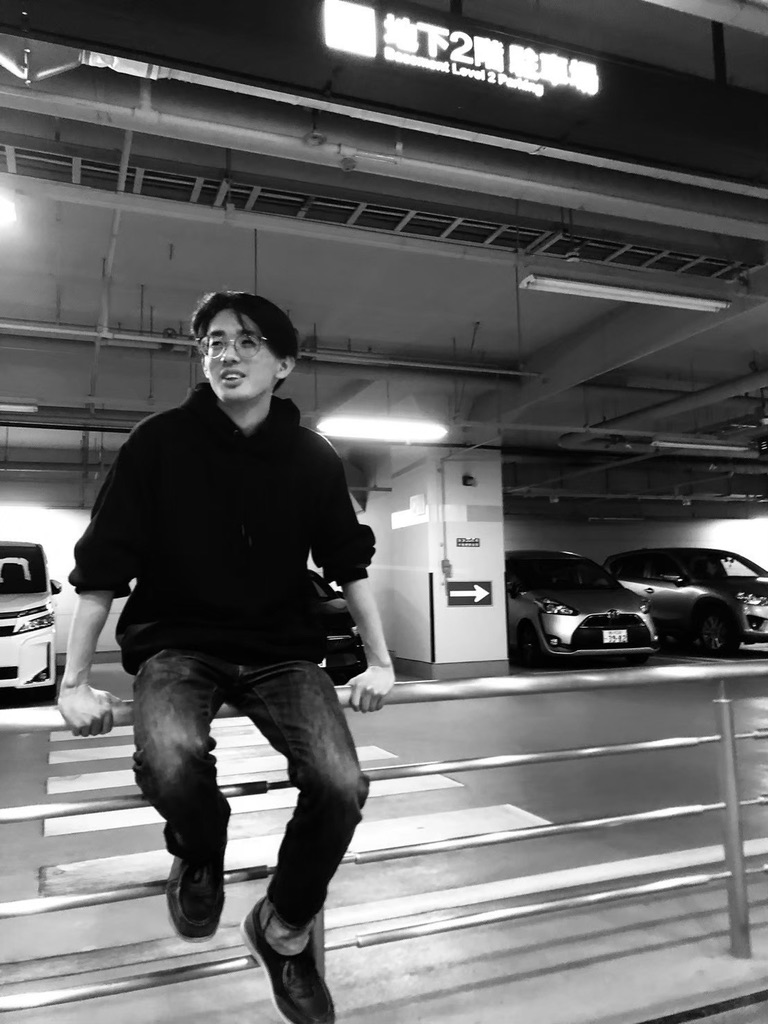
\includegraphics[width=1.2\linewidth]{38A299D4-7495-44B7-B699-E1AF92AFC245_1_105_c.jpeg}
        \end{column}
    \end{columns}
\end{frame}

\begin{frame}{このセミナーで目指すもの}
    \begin{goal}
        量子力学における自発的対称性の破れを理解する
    \end{goal}

    
\includegraphics[width=0.1\linewidth]{Nobel_prize_medal.svg.png}
    南部陽一郎・小林誠・益川敏英 ノーベル賞(2008)
\end{frame}

\begin{frame}{このセミナーで登場しないもの}
    \begin{itemize}
        \item 実験事実
        \item 波動関数
        \item シュレディンガー方程式
        \item 微積分
        \item 三角関数
    \end{itemize}
\end{frame}

\begin{frame}{なぜ「物理」をやらないのか?}
    \begin{enumerate}
        \item 現象が\alert{\textbf{直観とかけ離れている}}
        \begin{itemize}
            \item 状態の重ね合わせ?
            \item 測定したら状態が変わる?
            \item 位置と速度が同時に決まらない?
            \item 量子もつれ?
        \end{itemize}
        \item \alert{\textbf{学部1年の線形代数だけ}}で理解できる
        \begin{itemize}
            \item 複素ベクトル
            \item エルミート行列
            \item ユニタリ行列
        \end{itemize}
    \end{enumerate}
    難しそうだが、全て\textbf{\red{たしざんとかけざん}}。

    \textbf{計算できるようになると、なぜか量子力学の感覚を掴めてくる}
\end{frame}



\section{べくとるとぎょーれつ}

% \subsection{たしざん・かけざんのふくしゅう}


\subsection{べくとる}

\begin{frame}{ベクトル}
    ベクトルは数がいっぱい並んだもの。
    4つ数が並ぶと4次元。

    量子力学のお約束に従って、ブラ・ケットで書くと、後々直感的にわかりやすい。
    \begin{equation*}
        \ket{1,2,4,3}
        =
        \mqty[1\\2\\4\\3]
        =
        \vcenter{\hbox{
            \begin{tikzpicture}
                \node at(0,0)[draw,rectangle](ket){$\ket{1,2,4,3}$};
                \draw(ket.west)--++(-.5,0);
            \end{tikzpicture}
        }}
    \end{equation*}
    \begin{equation*}
        \bra{1,2,4,3}
        =
        \mqty[1&2&4&3]
        =
        \vcenter{\hbox{
            \begin{tikzpicture}
                \node at(0,0)[draw,rectangle](ket){$\bra{1,2,4,3}$};
                \draw(ket.east)--++(.5,0);
            \end{tikzpicture}
        }}
    \end{equation*}
    量子力学ではベクトルは状態を表すので、\alert{\textbf{状態ベクトル}}と呼ぶことにする。
\end{frame}

\begin{frame}{状態ベクトルの足し算}
    同じ次元のブラ同士、ケット同士なら単純に足すだけ。
    \begin{equation*}
        \mqty[1\\2\\4\\3]
        +
        \mqty[5\\3\\1\\4]
        =
        \mqty[6\\5\\5\\7]
    \end{equation*}
    次元が違うもの、ブラとケットは足せない。

    足し算の延長でスカラー倍もそのまま。
    \begin{equation*}
        3\mqty[1\\2\\4\\3]
        =
        \mqty[3\\6\\12\\9]
    \end{equation*}
\end{frame}

\begin{frame}{状態ベクトルどうしの掛け算 (内積)}
    \begin{equation*}
        \begin{split}
            \mqty[\red{1} & \blue{2} & \green{4} & 3]
            \mqty[\red{5} \\ \blue{1} \\ \green{-3}\\ 2]
            &=
            \red{1\cdot5}
            +
            \blue{2\cdot1}
            +
            \green{4\cdot(-3)}
            +
            3\cdot2
            \\
            &=
            1
        \end{split}
    \end{equation*}
    具体的な計算をしないなら、お絵描きしたほうがわかりやすい。
    \begin{equation*}
        \vcenter{\hbox{
            \begin{tikzpicture}
                \node at(0,0)[draw,rectangle](ket){$\ket{5,1,-3,2}$};
                \node at(-3,0)[draw,rectangle](bra){$\bra{1,2,4,3}$};
                \draw(bra.east)--(ket.west);
            \end{tikzpicture}
        }}
        =
        1
    \end{equation*}
    脚が出てないので状態ベクトルじゃない。
\end{frame}

% \begin{frame}{一方その頃量子力学では}
%     量子力学では, すべての情報はベクトルが持っている.

%     状態ベクトル=状態。
%     \begin{prop*}{測定により$\ket{\psi}$が測定される確率}{}
%         \begin{equation*}
%             P_\psi
%             \propto
%             \braket{\psi}
%             =
%             \vcenter{\hbox{
%                 \begin{tikzpicture}
%                     \node at(0,0)[draw,rectangle](ket){$\ket{\psi}$};
%                     \node at(-1,0)[draw,rectangle](bra){$\bra{\psi}$};
%                     \draw(bra.east)--(ket.west);
%                 \end{tikzpicture}
%             }}
%         \end{equation*}
%     \end{prop*}

%     状態って???

%     $\rightarrow$詳しい話はこの後
% \end{frame}


\subsection{たしざん・かけざんがいっぱい}

\begin{frame}{行列の状態ベクトルへの作用}
    \begin{equation*}
        \mqty[\red{1} & \blue{2} \\ \green{-1} & \purple{4}]
        \mqty[1 \\ -2]
        =
        \mqty[
            \red{1}\cdot1+\blue{2}\cdot(-2)
            \\
            \green{-1}\cdot1+\purple{4}\cdot(-2)
        ]
        =
        \mqty[-3\\-9]
    \end{equation*}
    こういうのを
    \begin{equation*}
        \hat{H}\ket{\psi}
        =
        \ket{H\psi}
    \end{equation*}
    \begin{equation*}
        \vcenter{\hbox{
            \begin{tikzpicture}
                \node at(0,0)[draw, rectangle](H){$\hat{H}$};
                \node at(1,0)[draw, rectangle](psi){$\ket{\psi}$};
                \draw(H.east)--(psi.west)(H.west)--++(-.5,0);
            \end{tikzpicture}
        }}
        =
        \vcenter{\hbox{
            \begin{tikzpicture}
                \node at(1,0)[draw, rectangle](psi){$\ket{H\psi}$};
                \draw(psi.west)--++(-.5,0);
            \end{tikzpicture}
        }}
    \end{equation*}
    みたいに書く。
    $\hat{H}$は状態ベクトルを状態ベクトルにするので脚が2本。
    \begin{equation*}
        \hat{H}
        =
        \vcenter{\hbox{
            \begin{tikzpicture}
                \node at(0,0)[draw,rectangle](H){$\hat{H}$};
                \draw(H.east)--++(.5,0);
                \draw(H.west)--++(-.5,0);
            \end{tikzpicture}
        }}
    \end{equation*}
\end{frame}

\begin{frame}{矢印で理解するなら}
    % \begin{equation*}
    %     \mqty[a & b \\ c & d]\mqty[e_x \\ e_y]
    %     =
    %     \mqty[ae_x+be_y \\ ce_x+de_y]
    % \end{equation*}
    \begin{equation*}
        \mqty[a & b \\ c & d]:
        \qty(\red{\mqty[1 \\ 0]}, \blue{\mqty[0 \\ 1]})
        \mapsto
        \qty(\red{\mqty[a \\ c]}, \blue{\mqty[b \\ d]})
    \end{equation*}
    ベクトルを回転・伸縮
    \begin{equation*}
        \vcenter{\hbox{
            \begin{tikzpicture}
                \draw[thin, dotted](-1,-1)grid(2,2);
                \draw[->, >=Stealth](-1,0)--(2,0);
                \draw[->, >=Stealth](0,-1)--(0,2);
                \draw[ultra thick, ->, red](0,0)--(1,0);
                \draw[ultra thick, ->, blue](0,0)--(0,1);
            \end{tikzpicture}
        }}
        \mapsto
        \vcenter{\hbox{
            \begin{tikzpicture}
                \draw[thin, dotted](1,2)--(-.5,-1);
                \draw[thin, dotted](-1,0)--(0,2);
                \draw[thin, dotted](2,2)--(.5,-1);
                \draw[thin, dotted](2,0)--(1.5,-1);
                \draw[thin, dotted](-1,2)--++(3,0);
                \draw[thin, dotted](-1,0)--++(3,0);
                \draw[ultra thick, ->, red](0,0)--(1,2);
                \draw[ultra thick, ->, blue](0,0)--(-1,0);
            \end{tikzpicture}
        }}
    \end{equation*}
\end{frame}

\begin{frame}{行列積}
    \begin{equation*}
        \begin{split}
            &
            \mqty[
                a & b
                \\
                c & d
            ]
            \mqty[
                e & f
                \\
                g & h
            ]
            \mqty[\alpha \\ \beta]
            =
            \mqty[
                a & b
                \\
                c & d
            ]
            \mqty[
                e\alpha+f\beta
                \\
                g\alpha+h\beta
            ]
            \\
            &=
            \mqty[
                a(e\alpha+f\beta)+b(g\alpha+h\beta)
                \\
                c(e\alpha+f\beta)+d(g\alpha+h\beta)
            ]
            \\
            &=
            \mqty[
                (ae+bg)\alpha+(af+bh)\beta
                \\
                (ce+dg)\alpha+(cf+dh)\beta
            ]
            \\
            &=
            \mqty[
                ae+bg & af+bh
                \\
                ce+dg & cf+dh
            ]
            \mqty[\alpha \\ \beta]
        \end{split}
    \end{equation*}
    \begin{equation*}
        \mqty[
            a & b
            \\
            c & d
        ]
        \mqty[
            e & f
            \\
            g & h
        ]
        =
        \mqty[
            ae+bg & af+bh
            \\
            ce+dg & cf+dh
        ]
    \end{equation*}
    \begin{equation*}
        \vcenter{\hbox{
            \begin{tikzpicture}
                \node at(0,0)[draw,rectangle](A){$\hat{A}$};
                \node at(1,0)[draw,rectangle](B){$\hat{B}$};
                \draw(A.east)--(B.west);
                \draw(A.west)--++(-.5,0);
                \draw(B.east)--++(.5,0);
            \end{tikzpicture}
        }}
        =
        \vcenter{\hbox{
            \begin{tikzpicture}
                \node at(0,0)[draw,rectangle](A){$\widehat{AB}$};
                \draw(A.west)--++(-.5,0);
                \draw(A.east)--++(.5,0);
            \end{tikzpicture}
        }}
    \end{equation*}
\end{frame}

\begin{frame}{行列積}
    \begin{equation*}
        \begin{split}
            &
            \mqty[
                A_{11} & A_{12} & \cdots & A_{1N}
                \\
                A_{\red{2}1} & A_{\red{2}2} & \cdots & A_{\red{2}N}
                \\
                \vdots & \vdots & \ddots & \vdots
                \\
                A_{N1} & A_{N2} & \cdots & A_{NN}
            ]
            \mqty[
                B_{1\blue{1}} & B_{12} & \cdots & B_{1N}
                \\
                B_{2\blue{1}} & B_{22} & \cdots & B_{2N}
                \\
                \vdots & \vdots & \ddots & \vdots
                \\
                B_{N\blue{1}} & B_{N2} & \cdots & B_{NN}
            ]
            \\
            &=
            \mqty[
                A_{11}B_{11}+\cdots+A_{1N}B_{N1} & \cdots & A_{11}B_{1N}+\cdots+A_{1N}B_{NN}
                \\
                A_{\red{2}1}B_{1\blue{1}}+\cdots+A_{\red{2}N}B_{N\blue{1}} & \cdots & A_{21}B_{1N}+\cdots+A_{2N}B_{NN}
                \\
                \vdots & \ddots & \vdots
                \\
                A_{N1}B_{11}+\cdots+A_{NN}B_{N1} & \cdots & A_{N1}B_{1N}+\cdots+A_{NN}B_{NN}
            ]
        \end{split}
    \end{equation*}
    \begin{equation*}
        (AB)_{\red{i}\blue{j}}
        =
        A_{\red{i}1}B_{1\blue{j}}+\cdots+A_{\red{i}N}B_{N\blue{j}}
    \end{equation*}

    むずそうなことやってるけど、結局は足し算と掛け算がいっぱいあるだけ。
\end{frame}

\begin{frame}{矢印で理解するなら}
    2回の回転・伸縮を合成
    \begin{equation*}
        \vcenter{\hbox{
            \begin{tikzpicture}
                \draw[thin, dotted](-1,-1)grid(2,2);
                \draw[->, >=Stealth](-1,0)--(2,0);
                \draw[->, >=Stealth](0,-1)--(0,2);
                \draw[ultra thick, ->, red](0,0)--(1,0);
                \draw[ultra thick, ->, blue](0,0)--(0,1);
            \end{tikzpicture}
        }}
        \mapsto
        \vcenter{\hbox{
            \begin{tikzpicture}
                \draw[thin, dotted](1,2)--(-.5,-1);
                \draw[thin, dotted](-1,0)--(0,2);
                \draw[thin, dotted](2,2)--(.5,-1);
                \draw[thin, dotted](2,0)--(1.5,-1);
                \draw[thin, dotted](-1,2)--++(3,0);
                \draw[thin, dotted](-1,0)--++(3,0);
                \draw[ultra thick, ->, red](0,0)--(1,2);
                \draw[ultra thick, ->, blue](0,0)--(-1,0);
            \end{tikzpicture}
        }}
        \mapsto
        \vcenter{\hbox{
            \begin{tikzpicture}
                \draw[thin, dotted](-1,-1)--(2,.5);
                \draw[thin, dotted](-1,-.5)--(2,1);
                \draw[thin, dotted](-1,0)--(2,1.5);
                \draw[thin, dotted](-1,.5)--(2,2);
                \draw[thin, dotted](-1,1)--(1,2);
                \draw[thin, dotted](-1,1.5)--(0,2);
                \draw[thin, dotted](0,-1)--(2,0);
                \draw[thin, dotted](1,-1)--(2,-.5);
                \draw[thin, dotted](-1,-1)--++(0,3);
                \draw[thin, dotted](0,-1)--++(0,3);
                \draw[thin, dotted](1,-1)--++(0,3);
                \draw[thin, dotted](2,-1)--++(0,3);
                \draw[ultra thick, ->, blue](0,0)--(0,.5);
                \draw[ultra thick, ->, red](0,0)--(1,.5);
            \end{tikzpicture}
        }}
    \end{equation*}
\end{frame}

% \begin{frame}{一方その頃量子力学では}
%     状態を変換すると別の状態になる
%     \begin{itemize}
%         \item 回転する
%         \item ズラす
%         \item 交換する
%     \end{itemize}
%     状態ベクトルを状態ベクトルに移すので、行列による作用で表せる
%     \begin{equation*}
%         \vcenter{\hbox{
%             \begin{tikzpicture}
%                 \node at(1,0)[draw, rectangle](psi){$\ket{\psi}$};
%                 \draw(psi.west)--++(-.5,0);
%             \end{tikzpicture}
%         }}
%         \mapsto
%         \vcenter{\hbox{
%             \begin{tikzpicture}
%                 \node at(0,0)[draw, rectangle](H){$\hat{U}$};
%                 \node at(1,0)[draw, rectangle](psi){$\ket{\psi}$};
%                 \draw(H.east)--(psi.west)(H.west)--++(-.5,0);
%             \end{tikzpicture}
%         }}
%     \end{equation*}
% \end{frame}


\section{こゆーほーてーしき}

\subsection{定義}

\begin{frame}{わかる人には一発でわからせる固有方程式}
    \begin{defn}[固有方程式]
        \begin{equation*}
            \mqty[
                H_{11} & \cdots & H_{1N}
                \\
                \vdots & \ddots & \vdots
                \\
                H_{N1} & \cdots & H_{NN}
            ]
            \underset{\red{\text{固有状態ベクトル}}}{
                \mqty[
                    \phi_1 \\ \vdots \\ \phi_N
                ]
            }
            =
            \underset{\red{\text{固有値}}}{E}
            \underset{\red{\text{固有状態ベクトル}}}{
                \mqty[
                    \phi_1 \\ \vdots \\ \phi_N
                ]
            }
        \end{equation*}
        \begin{equation*}
            \hat{H}\ket{\phi}
            =
            E\ket{\phi}
        \end{equation*}
        \begin{equation*}
            \vcenter{\hbox{
                \begin{tikzpicture}
                    \node at(-1,0)[draw,rectangle](H){$H$};
                    \node at(0,0)[draw,rectangle](psi){$\ket{\phi}$};
                    \draw(H.east)--(psi.west)(H.west)--++(-.5,0);
                \end{tikzpicture}
            }}
            =
            E
            \vcenter{\hbox{
                \begin{tikzpicture}
                    \node at(0,0)[draw,rectangle](psi){$\ket{\phi}$};
                    \draw(psi.west)--++(-.5,0);
                \end{tikzpicture}
            }}
        \end{equation*}
    \end{defn}
\end{frame}

\begin{frame}{固有方程式 定義のポイント}
    \begin{equation*}
        \vcenter{\hbox{
            \begin{tikzpicture}
                \node at(-1,0)[draw,rectangle](H){$H$};
                \node at(0,0)[draw,rectangle](psi){$\ket{\phi}$};
                \draw(H.east)--(psi.west)(H.west)--++(-.5,0);
            \end{tikzpicture}
        }}
        =
        E
        \vcenter{\hbox{
            \begin{tikzpicture}
                \node at(0,0)[draw,rectangle](psi){$\ket{\phi}$};
                \draw(psi.west)--++(-.5,0);
            \end{tikzpicture}
        }}
    \end{equation*}
    \begin{itemize}
        \item 両辺の固有状態ベクトル$\ket{\phi}$は同じ
        \item 固有値$E$はただの実数
    \end{itemize}
    $H$を決めると$(E, \ket{\phi})$の組が (一般には複数個) 出現
\end{frame}

\subsection{例}

\begin{frame}{例}
    \begin{equation*}
        \hat{H}
        =
        \mqty[
            1 & 0
            \\
            0 & -1
        ]
        \Longrightarrow
        (E,\ket{\phi})
        =
        \qty(1,\mqty[1\\0]),
        \qty(-1,\mqty[0\\1])
    \end{equation*}
    \begin{equation*}
        \hat{H}
        =
        \mqty[
            0 & 1
            \\
            1 & 0
        ]
        \Longrightarrow
        (E,\ket{\phi})
        =
        \qty(1,\mqty[1/\sqrt{2}\\1/\sqrt{2}]),
        \qty(1,\mqty[1/\sqrt{2}\\-1/\sqrt{2}])
    \end{equation*}
\end{frame}

\begin{frame}{手を動かせ}
    \begin{example}[$2\times2$でやってみよう!]
        \begin{equation*}
            \mqty[0 & 1 \\ 1 & 0]
            \mqty[1 \\ 1]
            =
            \mqty[0\cdot1+1\cdot1 \\ 1\cdot1+0\cdot1]
            =
            \mqty[1 \\ 1]
        \end{equation*}
        \begin{equation*}
            \mqty[0 & 1 \\ 1 & 0]
            \mqty[1 \\ -1]
            =
            \mqty[0\cdot1+1\cdot(-1) \\ 1\cdot1+0\cdot(-1)]
            =
            -\mqty[1 \\ -1]
        \end{equation*}
    \end{example}
    一般に行列$\hat{H}$から固有値$E$と固有状態ベクトル$\ket{\phi}$を見つけるのは至難の業
    (原理的にはできるが計算が膨大)。
\end{frame}

\begin{frame}{矢印で理解するなら}
    $\hat{H}\ket{\phi}=E\ket{\phi}$
    方向が変わらないベクトルが固有ベクトル。
    \begin{equation*}
        \vcenter{\hbox{
            \begin{tikzpicture}
                \draw[->, >=Stealth, ultra thick, red](0,0)--(1,0);
                \draw[->, >=Stealth, ultra thick, blue](0,0)--(0,1);
                \draw[->, >=Stealth, ultra thick](0,0)--(1,1);
            \end{tikzpicture}
        }}
        \mapsto
        \vcenter{\hbox{
            \begin{tikzpicture}
                \draw[->, >=Stealth, ultra thick, blue](0,0)--(1,2);
                \draw[->, >=Stealth, ultra thick, red](0,0)--(2,1);
                \draw[->, >=Stealth, ultra thick](0,0)--({sqrt(5)},{sqrt(5)});
            \end{tikzpicture}
        }}
    \end{equation*}

\end{frame}

\subsection{対角化と縮退}

% \begin{frame}{対角化}
%     以下我々が扱う行列は固有値が斜めに並んだだけの行列で表せることが知られている。
%     \begin{example}
%         固有値が$\{1,5,7\}$の行列はうまく変形することで
%         \begin{equation*}
%             \mqty[\dmat{1,5,7}]
%         \end{equation*}
%         の形になる。
%         固有値, 固有ベクトルは
%         \begin{equation*}
%             \qty(1, \mqty[1 \\ 0 \\ 0]),
%             \qquad
%             \qty(5, \mqty[0 \\ 1 \\ 0]),
%             \qquad
%             \qty(7, \mqty[0 \\ 0 \\ 1]).
%         \end{equation*}
%     \end{example}
% \end{frame}

\begin{frame}{異なる固有値の内積}
    \begin{them}
        固有値が異なる固有ベクトルは直交
    \end{them}
    \begin{equation*}
        \begin{split}
            o_1\braket{o_1}{o_2}
            &=
            (\bra{o_1}\hat{O})\ket{o_2}
            \\
            &=
            \bra{o_1}(\hat{O}\ket{o_2})
            =
            o_2\braket{o_1}{o_2}
        \end{split}
    \end{equation*}
    \begin{equation*}
        \therefore
        (o_1-o_2)\braket{o_1}{o_2}=0.
    \end{equation*}
    $o_1\neq o_2$では$\braket{o_1}{o_2}=0$.
\end{frame}

\begin{frame}{理論}
    \begin{defn}[理論]
        「エネルギー」を固有値にもつ行列$\hat{H}$
    \end{defn}
    \begin{equation*}
        \vcenter{\hbox{
            \begin{tikzpicture}
                \node at(0,0)[draw,rectangle, red](H){$\red{\hat{H}}$};
                \node at(1,0)[draw,rectangle](psi){$\ket{E}$};
                \draw(H.west)--++(-.5,0)(H.east)--(psi.west);
            \end{tikzpicture}
        }}
        =
        \underset{\text{エネルギー}}{E}
        \vcenter{\hbox{
            \begin{tikzpicture}
                \node at(1,0)[draw,rectangle](psi){$\ket{E}$};
                \node at(psi.south)[anchor=north, font=\scriptsize]{エネルギー固有状態};
                \draw(psi.west)--++(-.5,0);
            \end{tikzpicture}
        }}
    \end{equation*}
    エネルギーを求めたければ、
    \begin{equation*}
        \frac{
            \vcenter{\hbox{
                \begin{tikzpicture}
                    \node at(0,0)[draw,rectangle](H){$\hat{H}$};
                    \node at(1,0)[draw,rectangle](ket){$\ket{\psi}$};
                    \node at(-1,0)[draw,rectangle](bra){$\bra{\psi}$};
                    \draw(bra.east)--(H.west)(H.east)--(ket.west);
                \end{tikzpicture}
            }}
        }{
            \vcenter{\hbox{
                \begin{tikzpicture}
                    \node at(1,0)[draw,rectangle](ket){$\ket{\psi}$};
                    \node at(-1,0)[draw,rectangle](bra){$\bra{\psi}$};
                    \draw(bra.east)--(ket.west);
                \end{tikzpicture}
            }}
        }
        =E
    \end{equation*}
\end{frame}

\begin{frame}{縮退}
    \begin{defn}{縮退}
        状態$\ket{E;1},\ket{E;2}$が共に$\hat{H}$の固有値$E$の固有状態ベクトルでありながら
        \begin{equation*}
            \ket{E;1}
            \not\equiv
            \ket{E;2}
        \end{equation*}
        を満たすとき、$\ket{E;1}, \ket{E;2}$は\red{\textbf{縮退}}するという。
    \end{defn}
\end{frame}

\begin{frame}{縮退: 例}
    \begin{example}
        \begin{equation*}
            \hat{H}
            =
            \mqty[0 & 1 & 0 \\ 1 & 0 & 0 \\ 0 & 0 & 1]
        \end{equation*}
        の固有値・固有ベクトルは
        \begin{equation*}
            \qty(E,\ket{E})
            =
            \qty(1,\mqty[1 \\ 1 \\ 0]),
            \quad
            \qty(1,\mqty[0 \\ 0 \\ 1]),
            \quad
            \qty(-1,\mqty[1 \\ -1 \\ 0]).
        \end{equation*}
        \begin{equation*}
            \mqty[1 \\ 1 \\ 0]
            \not\equiv
            \mqty[0 \\ 0 \\ 1]
        \end{equation*}
    \end{example}
\end{frame}


\section{りろんたいけー}

\subsection{要請}

\begin{frame}{要請}
    \begin{requirement}
        \begin{enumerate}
            \item 「物理量」が\red{\textbf{一般には複数だが限定された}}「測定値」を持つ
            \item どんな「物理量」にも\red{\textbf{「測定値」がただ一つしか生じない}}状態ベクトルが存在する
            \item 任意の状態ベクトルは「測定値」がただ一つしか生じない状態ベクトルたちの\red{\textbf{重ね合わせ}}で書ける
            \item ある状態ベクトルの「測定値」が出る確率は、その「測定値」がただ一つしか生じない要請2の状態ベクトルと元の状態ベクトルだけで計算できる
        \end{enumerate}
    \end{requirement}
    何を言ってるかわからないと思うので説明します。
\end{frame}

\begin{frame}{要請1}
    \begin{requirement}
        「物理量」が\red{\textbf{一般には複数だが限定された}}「測定値」を持つ
    \end{requirement}
    ある状態ベクトルに「測定」を施すと、「測定値」セットのうちどれかが出てくる。
    \begin{figure}
        \centering
        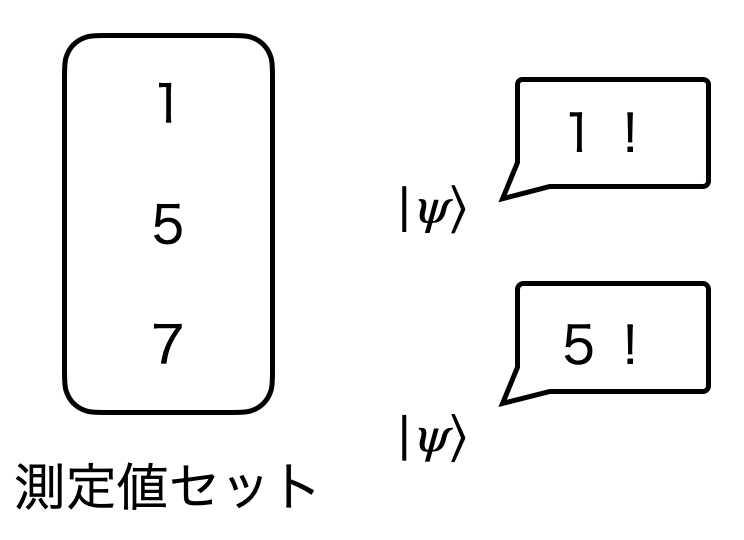
\includegraphics[width=5cm]{measurement.png}
    \end{figure}
    一般に測定ごとに結果が変わる。
\end{frame}

\begin{frame}{要請2}
    \begin{requirement}
        どんな「物理量」にも\red{\textbf{「測定値」がただ一つしか生じない}}状態ベクトルが存在する
    \end{requirement}
    何回「測定」を繰り返しても「測定値セット」のうちの1つだけしか出てこない。
    \begin{figure}
        \centering
        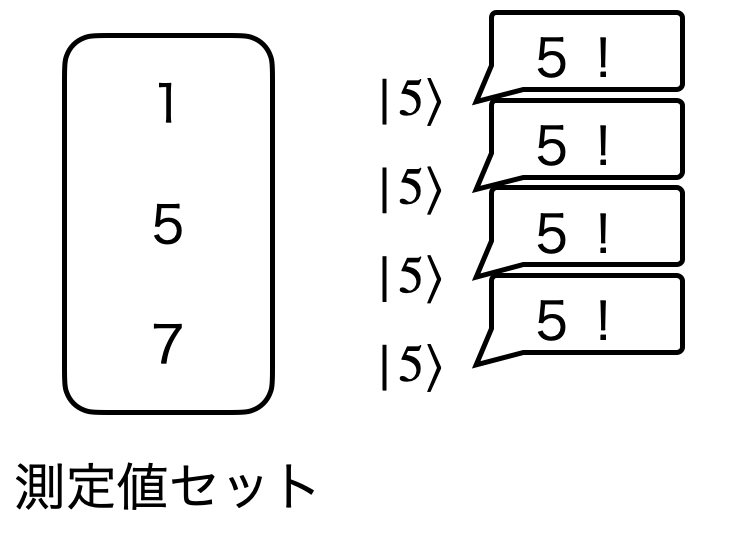
\includegraphics[width=5cm]{eigenmeasurement.png}
    \end{figure}
\end{frame}

\begin{frame}{要請3}
    \begin{requirement}
        任意の状態ベクトルは「測定値」がただ一つしか生じない状態ベクトルたちの\red{\textbf{重ね合わせ}}で書ける
    \end{requirement}
    \begin{equation*}
        \text{測定値}=\{1, 5, 7\}
        \Longrightarrow
        \ket{\psi}=c_1\ket{1}+c_5\ket{5}+c_7\ket{7}
    \end{equation*}
    こういうのを「$\ket{1}, \ket{5}, \ket{7}$を混ぜる」とか言います。
\end{frame}

\begin{frame}{要請4}
    \begin{requirement}
        ある状態ベクトルの「測定値」が出る確率は、その「測定値」がただ一つしか生じない要請2の状態ベクトルと元の状態ベクトルだけで計算できる。
    \end{requirement}
    状態ベクトル$\ket{\psi}$で測定値セット$\{1, 5, 7\}$のうち$5$が出る確率

    $\longleftarrow$
    $\ket{\psi}$ \& $\ket{5}$で計算可能。
\end{frame}


\subsection{物理量の評価}

\begin{frame}{物理量の表し方}
    \begin{enumerate}
        \item 物理量を、測定値が固有値の行列で表す
        \item 要請3『任意の状態ベクトルは「測定値」がただ一つしか生じない状態ベクトルたちの\textbf{重ね合わせ}で書ける』に従って、状態ベクトルを分解
        \item 分解した固有状態ベクトルの固有値が測定値になり得る
    \end{enumerate}
    \begin{example}
        固有値$\{1,5,7\}$の物理量を状態
        \begin{equation*}
            \ket{\psi}
            =
            c_1\ket{1}+c_5\ket{5}
        \end{equation*}
        で測定すると、測定値は1 or 5.
    \end{example}
\end{frame}

\begin{frame}{特定の測定値を出す確率}
    物理量$\hat{O}$の固有値$\{o_1,o_2,\dots\}$とその固有ベクトル$\{\ket{o_1}, \ket{o_2}, \dots\}$.
    \begin{defn}
        状態$\ket{\psi}$で$\hat{O}$を測定して測定値$o_1$が出る確率:
        \begin{equation*}
            P_{o_1}=\frac{|\braket{o_1}{\psi}|^2}{\braket{\psi}\braket{o_1}}
            =
            \frac{
                \qty|
                    \vcenter{\hbox{
                        \begin{tikzpicture}
                            \node at(0,0)[draw,rectangle](o){$\bra{o_1}$};
                            \node at(1,0)[draw,rectangle](psi){$\ket{\psi}$};
                            \draw(o.east)--(psi.west);
                        \end{tikzpicture}
                    }}
                |^2
            }{
                \vcenter{\hbox{
                    \begin{tikzpicture}
                        \node at(0,0)[draw,rectangle](o){$\bra{\psi}$};
                        \node at(1,0)[draw,rectangle](psi){$\ket{\psi}$};
                        \draw(o.east)--(psi.west);
                    \end{tikzpicture}
                }}
                \vcenter{\hbox{
                    \begin{tikzpicture}
                        \node at(0,0)[draw,rectangle](o){$\bra{o_1}$};
                        \node at(1,0)[draw,rectangle](psi){$\ket{o_1}$};
                        \draw(o.east)--(psi.west);
                    \end{tikzpicture}
                }}
            }.
        \end{equation*}
    \end{defn}
    固有状態ベクトルでは100\%固有値が出る:
    \begin{equation*}
        P_{o_1}=\frac{|\braket{o_1}|^2}{\braket{o_1}\braket{o_1}}=1,
        \qquad
        P_{o_2}=\frac{|\braket{o_2}{o_1}|^2}{\braket{o_1}\braket{o_2}}=0.
    \end{equation*}
\end{frame}

\begin{frame}{期待値}
    \begin{defn}{期待値}
        \begin{equation*}
            \text{期待値}=\sum\text{値}\times\text{確率}
        \end{equation*}
    \end{defn}
    \begin{example}
        $|\braket{\psi}|=|\braket{o_1}|=1$の状態が$\ket{\psi}=c_1\ket{1}+c_5\ket{5}$なら、
        \begin{equation*}
            \begin{split}
                \ev{\hat{O}}{\psi}
                &=
                \vcenter{\hbox{
                    \begin{tikzpicture}
                        \node at (0,0)[draw,rectangle](O){$\hat{O}$};
                        \node at (-1,0)[draw,rectangle](left){$\bra{\psi}$};
                        \node at (1,0)[draw,rectangle](right){$\ket{\psi}$};
                        \draw(left.east)--(O.west)(O.east)--(right.west);
                    \end{tikzpicture}
                }}
                \\
                &=
                (\bra{1}c_1^\ast+\bra{5}c_5^\ast)\hat{O}(c_1\ket{1}+c_5\ket{5})
                \\
                &=
                |c_1|^2\ev{\hat{O}}{1}
                +
                c_1^\ast c_5\cdot5\bra{1}\ket{5}
                \\
                &\qquad
                +
                c_5^\ast c_1\cdot1\bra{5}\ket{1}
                +
                |c_5|^2\ev{\hat{O}}{5}
                \\
                &=
                1|\braket{1}{\psi}|^2
                +
                5|\braket{5}{\psi}|^2
                =
                1P_1+5P_5
            \end{split}
        \end{equation*}
    \end{example}
\end{frame}


\section{じはつてきたいしょーせーのやぶれ}

\subsection{対称性}

\begin{frame}{状態ベクトルの変換}
    \begin{requirement}{要請3}
        任意の状態ベクトルは「測定値」がただ一つしか生じない状態ベクトルたちの\textbf{\red{重ね合わせ}}で書ける
    \end{requirement}
    重ね合わせ=行列の状態ベクトルへの作用で、大きさを変えないもの
    \begin{equation*}
        \ket{\psi}
        \to
        \hat{U}\ket{\psi}
        =
        \ket{U\psi}
    \end{equation*}
    \begin{equation*}
        \vcenter{\hbox{
            \begin{tikzpicture}
                \node at(0,0)[draw, rectangle](U){$\hat{U}$};
                \node at(1,0)[draw, rectangle](psi){$\ket{\psi}$};
                \draw(U.west)--++(-.5,0)(U.east)--(psi.west);
            \end{tikzpicture}
        }}
    \end{equation*}
    \begin{equation*}
        \text{w/ }\braket{U\psi}=\braket{\psi}
    \end{equation*}
\end{frame}

\begin{frame}{例: 回転}
    \begin{equation*}
        \hat{U}_{45^\circ}
        =
        \frac{1}{\sqrt{2}}\mqty[1 & -1 \\ 1 & 1]
    \end{equation*}
    \begin{equation*}
        \vcenter{\hbox{
            \begin{tikzpicture}
                \draw[thin, dotted](-1,-1)grid(2,2);
                \draw[ultra thick, red, ->, >=Stealth](0,0)--(1,0);
                \draw[ultra thick, blue, ->, >=Stealth](0,0)--(0,1);
            \end{tikzpicture}
        }}
        \to
        \vcenter{\hbox{
            \begin{tikzpicture}[rotate=-45]
                \draw[thin, dotted, ->, >=Stealth](-1,-1)grid(2,2);
                \draw[ultra thick, red, ->, >=Stealth](0,0)--(0:1);
                \draw[ultra thick, blue, ->, >=Stealth](0,0)--(90:1);
            \end{tikzpicture}
        }}
    \end{equation*}
\end{frame}

\begin{frame}{状態の対称性}
    \begin{defn}[状態が変換$\hat{U}$で対称]
        \begin{equation*}
            \ket{\psi}
            \equiv
            \hat{U}\ket{\psi}
        \end{equation*}
    \end{defn}
    \begin{example}
        \begin{equation*}
            \ket{\leftrightarrow}
            :=
            \frac{\ket{\rightarrow}+\hat{U}_{180^\circ}\ket{\rightarrow}}{\sqrt{2}}
        \end{equation*}
        は$180^\circ$回転で不変
        \begin{equation*}
            \hat{U}_{180^\circ}\ket{\leftrightarrow}
            =
            \frac{\hat{U}_{180^\circ}\ket{\rightarrow}+\hat{U}_{360^\circ}\ket{\rightarrow}}{\sqrt{2}}
            \equiv
            \ket{\leftrightarrow}
        \end{equation*}
        $\longrightarrow180^\circ$回転対称
    \end{example}
\end{frame}

\begin{frame}{理論の対称性}
    もし\red{どの}エネルギー固有状態$\ket{E}$を$180^\circ$回転した$\ket{UE}=\hat{U}_{180^\circ}\ket{E}$もエネルギーが変わらないなら、
    \begin{equation*}
        \begin{split}
            \vcenter{\hbox{
                \begin{tikzpicture}
                    \node at(0,0)[draw,rectangle](U){$\hat{U}$};
                    \node at(1,0)[draw,rectangle](H){$\hat{H}$};
                    \node at(2,0)[draw,rectangle](E){$\ket{E}$};
                    \draw(U.west)--++(-.5,0)(U.east)--(H.west)(H.east)--(E.west);
                \end{tikzpicture}
            }}
            &=
            E
            \vcenter{\hbox{
                \begin{tikzpicture}
                    \node at(0,0)[draw,rectangle](U){$\hat{U}$};
                    \node at(1,0)[draw,rectangle](E){$\ket{E}$};
                    \draw(U.west)--++(-.5,0)(U.east)--(E.west);
                \end{tikzpicture}
            }}
            \\
            &=
            E
            \vcenter{\hbox{
                \begin{tikzpicture}
                    \node at(0,0)[draw,rectangle](U){$\ket{UE}$};
                    % \node at(1,0)[draw,rectangle](E){$\ket{UE}$};
                    \draw(U.west)--++(-.5,0);
                \end{tikzpicture}
            }}
            \\
            &\equiv
            \vcenter{\hbox{
                \begin{tikzpicture}
                    \node at(0,0)[draw,rectangle](U){$\ket{UE}$};
                    \node at(-1,0)[draw,rectangle](H){$\hat{H}$};
                    \draw(H.west)--++(-.5,0)(H.east)--(U.west);
                \end{tikzpicture}
            }}
            \\
            &=
            \vcenter{\hbox{
                \begin{tikzpicture}
                    \node at(0,0)[draw,rectangle](U){$\hat{H}$};
                    \node at(1,0)[draw,rectangle](H){$\hat{U}$};
                    \node at(2,0)[draw,rectangle](E){$\ket{E}$};
                    \draw(U.west)--++(-.5,0)(U.east)--(H.west)(H.east)--(E.west);
                \end{tikzpicture}
            }}
        \end{split}
    \end{equation*}
    \begin{defn}[理論の対称性]
        $\hat{H}\hat{U}=\hat{U}\hat{H}$
        $\Longleftrightarrow$理論$\hat{H}$は$\hat{U}$で対称
    \end{defn}
\end{frame}

\begin{frame}{例}
    \begin{example}
        \begin{equation*}
            \hat{H}=\mqty[\dmat{1,-1,-1,1}],
            \qquad
            \hat{U}=\mqty[ & & & 1 \\ & & 1 & \\ & 1 & & \\ 1 & & & ]
        \end{equation*}
        \begin{equation*}
            \hat{H}\hat{U}
            =
            \mqty[ & & & 1 \\ & & -1 & \\ & -1 & & \\ 1 & & & ]
            =
            \hat{U}\hat{H}
        \end{equation*}
        理論$\hat{H}$は変換$\hat{U}$を対称性にもつ。
    \end{example}
\end{frame}


\subsection{自発的対称性の破れ}

\begin{frame}{基底状態}
    \begin{defn}[基底状態]
        理論$\hat{H}$の最小固有値を出す固有状態$\ket{E_0}$
    \end{defn}
    \begin{example}
        \begin{equation*}
            \hat{H}=\mqty[ & 1 \\ 1 & ]
        \end{equation*}
        固有値(=エネルギーの測定値)は$\pm1$.
        最小のエネルギー$E=-1$を与える
        \begin{equation*}
            \ket{E_9}=\mqty[1 \\ -1]
        \end{equation*}
        が基底状態。
    \end{example}
    絶対零度では基底状態(の重ね合わせ)が実現する
\end{frame}

\begin{frame}{自発的対称性の破れ}
    変換$\hat{U}$, 理論$\hat{H}$, 状態$\ket{\mathrm{\psi}}$に対して、
    \begin{description}
        \item[状態の対称性] $\ket{\psi}\equiv\hat{U}\ket{\psi}$
        \item[理論の対称性] $\hat{H}\hat{U}=\hat{U}\hat{H}$
    \end{description}
    \begin{defn}[自発的対称性の破れ]
        理論は対称性を守っているが、基底状態が対称性を破っていること
    \end{defn}
    
\includegraphics[width=0.1\linewidth]{Nobel_prize_medal.svg.png}
    南部陽一郎・小林誠・益川敏英のノーベル賞(2008)
\end{frame}

\begin{frame}{自発的対称性の破れ: 例}
    \begin{example}
        \begin{equation*}
            \hat{H}
            =
            % \mqty[0 & -1 & 0 \\ -1 & 0 & 0 \\ 0 & 0 & -1]
            \mqty[\dmat{1,-1,-1}],
            \qquad
            \hat{U}
            =
            \mqty[1 & & \\ & & 1 \\ & 1 &]
        \end{equation*}
        $\hat{H}$の固有値は$\pm1$.
        基底状態は\red{\textbf{2つ}}。
        \begin{equation*}
            \ket{\uparrow}
            =
            \mqty[0 \\ 1 \\ 0],
            \qquad
            \ket{\downarrow}
            =
            \mqty[0 \\ 0 \\ 1].
        \end{equation*}
        $\hat{H}\hat{U}=\hat{U}\hat{H}$だが$\hat{U}\ket{\uparrow}=\ket{\downarrow}\not\equiv\ket{\uparrow}$.
        \textbf{\red{何が楽しい?}}
    \end{example}
\end{frame}

\begin{frame}{物理的直感}
    矢印の向きが揃った方が低エネルギーとする
    \begin{equation*}
        \vcenter{\hbox{
            \begin{tikzpicture}
                \draw(0,0)--(3,0);
                \foreach\x in{0,1,...,3}{
                    \draw[->, very thick](\x,-.5)--(\x,.5);
                }
            \end{tikzpicture}
        }}
        <
        \vcenter{\hbox{
            \begin{tikzpicture}
                \draw(0,0)--(3,0);
                \draw[->, very thick](0,-.5)--++(0,1);
                \draw[->, very thick](1,.5)--++(0,-1);
                \draw[->, very thick](2,-.5)--++(0,1);
                \draw[->, very thick](3,.5)--++(0,-1);
            \end{tikzpicture}
        }}
    \end{equation*}
    理論は「揃え」としか言っていないのに、実現する状態は揃う向きが勝手に決まる

    $\rightarrow$磁性の発現, 磁石のメカニズム
\end{frame}

\begin{frame}{相図}
    対称性がわかると結構わかる
    \begin{figure}
        \centering
        \begin{minipage}{0.45\linewidth}
            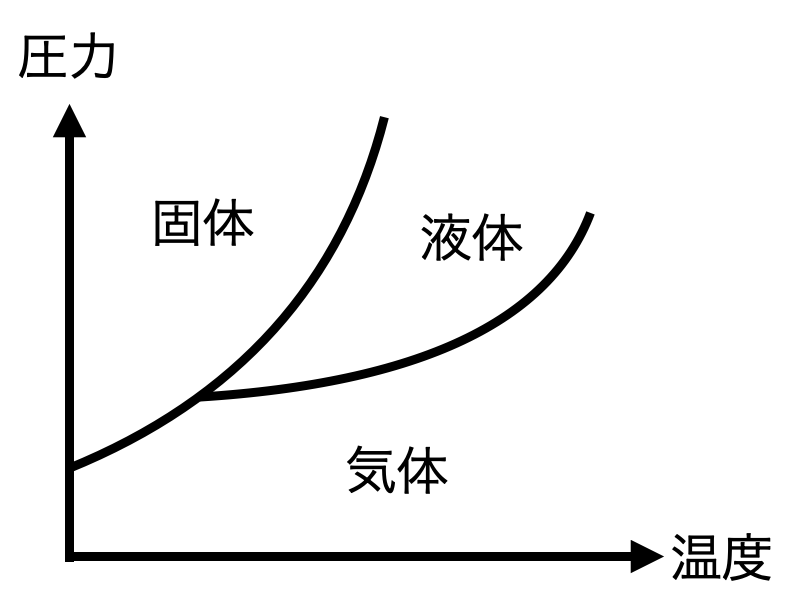
\includegraphics[width=0.8\linewidth]{phase3.png}
        \end{minipage}
        \begin{minipage}{0.45\linewidth}
            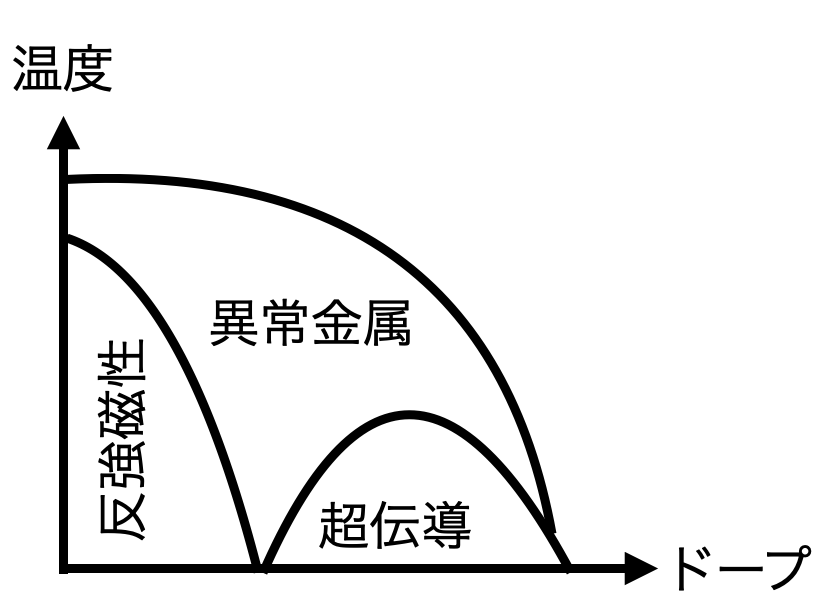
\includegraphics[width=0.8\linewidth]{phase-mag.png}
        \end{minipage}
    \end{figure}
    \textbf{自発的対称性の破れだけでほとんどの線が引ける}
\end{frame}

\begin{frame}{次回予告}
    相図の全ての線が自発的対称性の破れで書けると思っていた。

    そう、量子ホール効果の出現までは...

    次回\textbf{「トポロジカル秩序の分類に制限を与える禁止定理」}
\end{frame}

\begin{frame}{量子力学の参考書}
    \begin{itemize}
        \item \textbf{清水明「新版 量子論の基礎」サイエンス社}

        今回の流れに沿っている。
        数学的に厳密に寄せているのに、わかりやすい。
        初学者にも勧められる。
        \item \textbf{J. J. サクライ「現代の量子力学(上)」吉岡書店}

        今回つかったブラケット記法による有名書。
        ゼミに便利。
        一人で読むなら2冊目以降。
        \item \textbf{猪木慶治・川合光「量子力学I」講談社}

        今回扱わなかった波動関数表示で進める。
        割と王道。
    \end{itemize}
\end{frame}

\begin{frame}{2025年物性若手夏の学校やります!!!}
    \begin{itemize}
        \item 全国の物性物理関連の大学院生が集結
        \item 4泊5日の集中合宿
        \item 講義・集中ゼミで最先端研究をキャッチアップ
        \item 学会形式で自分の研究を発表
    \end{itemize}
    若手研究者が研究の道を本格的に歩み始める第一歩になります!!!

    \textbf{\red{参加・斡旋・各種協賛お願いします!!!}}

    \textbf{\red{$\downarrow$個人協賛応募フォーム$\downarrow$}}(調整中)
    \begin{figure}
        \centering
        
\includegraphics[width=0.3\linewidth]{QR_736654.png}
    \end{figure}
\end{frame}

\end{document}
